\section{Hatano-Nelson model: A flavor of non-Hermiticity in a lattice}
\begin{figure}[H]
    \centering 
    

\tikzset{every picture/.style={line width=0.75pt}} %set default line width to 0.75pt        

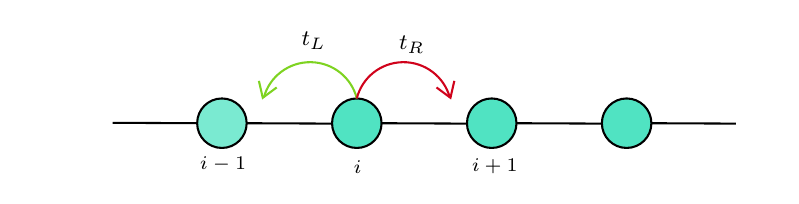
\begin{tikzpicture}[x=0.75pt,y=0.75pt,yscale=-1,xscale=1]
%uncomment if require: \path (0,109); %set diagram left start at 0, and has height of 109

%Shape: Circle [id:dp5679706103157838] 
\draw  [fill={rgb, 255:red, 80; green, 227; blue, 194 }  ,fill opacity=0.76 ] (212.15,71.93) .. controls (212.15,65.34) and (217.49,60) .. (224.07,60) .. controls (230.66,60) and (236,65.34) .. (236,71.93) .. controls (236,78.51) and (230.66,83.85) .. (224.07,83.85) .. controls (217.49,83.85) and (212.15,78.51) .. (212.15,71.93) -- cycle ;
%Straight Lines [id:da982381607909628] 
\draw    (236,71.93) -- (276.68,72.12) ;
%Shape: Circle [id:dp23206932607396458] 
\draw  [fill={rgb, 255:red, 80; green, 227; blue, 194 }  ,fill opacity=1 ] (277.15,71.93) .. controls (277.15,65.34) and (282.49,60) .. (289.07,60) .. controls (295.66,60) and (301,65.34) .. (301,71.93) .. controls (301,78.51) and (295.66,83.85) .. (289.07,83.85) .. controls (282.49,83.85) and (277.15,78.51) .. (277.15,71.93) -- cycle ;
%Straight Lines [id:da6300638154973164] 
\draw    (301,71.93) -- (341.68,72.12) ;
%Shape: Circle [id:dp9264939026993823] 
\draw  [fill={rgb, 255:red, 80; green, 227; blue, 194 }  ,fill opacity=1 ] (342.15,71.93) .. controls (342.15,65.34) and (347.49,60) .. (354.07,60) .. controls (360.66,60) and (366,65.34) .. (366,71.93) .. controls (366,78.51) and (360.66,83.85) .. (354.07,83.85) .. controls (347.49,83.85) and (342.15,78.51) .. (342.15,71.93) -- cycle ;
%Straight Lines [id:da9201072853916674] 
\draw    (366,71.93) -- (406.68,72.12) ;
%Shape: Circle [id:dp6666759085430102] 
\draw  [fill={rgb, 255:red, 80; green, 227; blue, 194 }  ,fill opacity=1 ] (407.15,71.93) .. controls (407.15,65.34) and (412.49,60) .. (419.07,60) .. controls (425.66,60) and (431,65.34) .. (431,71.93) .. controls (431,78.51) and (425.66,83.85) .. (419.07,83.85) .. controls (412.49,83.85) and (407.15,78.51) .. (407.15,71.93) -- cycle ;
%Straight Lines [id:da2140414629064964] 
\draw    (431,71.93) -- (471.68,72.12) ;
%Straight Lines [id:da7102278145283337] 
\draw    (171.47,71.73) -- (212.15,71.93) ;
%Shape: Arc [id:dp17908903300713808] 
\draw  [draw opacity=0] (244.31,59.39) .. controls (247.03,49.54) and (256.18,42.37) .. (266.94,42.52) .. controls (277.69,42.68) and (286.62,50.09) .. (289.07,60) -- (266.61,65.51) -- cycle ; \draw  [color={rgb, 255:red, 126; green, 211; blue, 33 }  ,draw opacity=1 ] (244.31,59.39) .. controls (247.03,49.54) and (256.18,42.37) .. (266.94,42.52) .. controls (277.69,42.68) and (286.62,50.09) .. (289.07,60) ;  
%Shape: Arc [id:dp4029984468712787] 
\draw  [draw opacity=0] (333.84,59.39) .. controls (331.12,49.54) and (321.97,42.37) .. (311.21,42.52) .. controls (300.46,42.68) and (291.53,50.09) .. (289.07,60) -- (311.54,65.51) -- cycle ; \draw  [color={rgb, 255:red, 208; green, 2; blue, 27 }  ,draw opacity=1 ] (333.84,59.39) .. controls (331.12,49.54) and (321.97,42.37) .. (311.21,42.52) .. controls (300.46,42.68) and (291.53,50.09) .. (289.07,60) ;  
\draw  [color={rgb, 255:red, 126; green, 211; blue, 33 }  ,draw opacity=1 ] (250.48,54.7) -- (243.77,59.67) -- (241.9,51.54) ;
\draw  [color={rgb, 255:red, 208; green, 2; blue, 27 }  ,draw opacity=1 ] (327.48,54.7) -- (334.19,59.67) -- (336.06,51.54) ;

% Text Node
\draw (148,69.8) node [anchor=north west][inner sep=0.75pt]    {$\dotsc $};
% Text Node
\draw (131,69.8) node [anchor=north west][inner sep=0.75pt]    {$\dotsc $};
% Text Node
\draw (486,69.8) node [anchor=north west][inner sep=0.75pt]    {$\dotsc $};
% Text Node
\draw (469,69.8) node [anchor=north west][inner sep=0.75pt]    {$\dotsc $};
% Text Node
\draw (261,26.4) node [anchor=north west][inner sep=0.75pt]  [font=\footnotesize]  {$t_{L}$};
% Text Node
\draw (308,28.4) node [anchor=north west][inner sep=0.75pt]  [font=\footnotesize]  {$t_{R}$};
% Text Node
\draw (286,88.4) node [anchor=north west][inner sep=0.75pt]  [font=\scriptsize]  {$i$};
% Text Node
\draw (343,87.63) node [anchor=north west][inner sep=0.75pt]  [font=\scriptsize]  {$i+1$};
% Text Node
\draw (212,86.63) node [anchor=north west][inner sep=0.75pt]  [font=\scriptsize]  {$i-1$};


\end{tikzpicture}

    \caption{Diagram showing the hopping in Hatano-Nelson Model}
\end{figure}%
The Hatano-Nelson model (non-disordered) is the simplest tight-binding
lattice model where the left and right-moving hopping amplitudes are unequal
(\emph{non-reciprocal}). The Hamiltonian for spinless particles in one dimension reads,
\blgn
 \hHN = \sum_{i=0}^{L-1} \big[t_R c\y_i c\py_{i+1} + t_L c\y_{i+1} c\py_i \big]\,,   
\elgn
where $L$ is the number of sites in the lattice and $t_R$ and $t_L$ are the right and left hopping
amplitudes. The Hamiltonian is written using the second quantisation formalism, where $c\py_i$ and  $c\y_i$ are the particle annihilation and
creation operators at lattice site $i$, respectively. {The Hamiltonian becomes non-Hermitian when $t_L\neq t_R$, that is, \textit{asymmetric hopping}.} 

We can express the anihilation operator in the momentum space as:
\blgn
c_{i} = \f{1}{\sqrt L}\sum_{k=0}^{L-1} e^{ikx_i} c_{k}.
\elgn 
where $x_i$ is the coordinate or position of site $i$. We then substitute this in the Hamiltonian:
\blgn
 \hHN&= \sum\limits_{L}\sum\limits_k\sum\limits_{k'} t_R e^{-ikx_i}e^{ik'(x_{i}+a)}  c\y_k c\py_{k'} +t_L e^{-ik(x_i+a)}e^{ik'x_{i}}  c\y_k c\py_{k'} \\
 &= \sum\limits_{L}\sum\limits_k\sum\limits_{k'} \qty(t_R e^{ix_i(k'-k)}e^{ik'a}+t_L e^{ix_i(k'-k)}e^{-ika})c\y_k c\py_{k'}\\
 &=\sum\limits_k \qty(t_Re^{ika} + t_Le^{-ika})c\y_k c\py_k \qquad\qquad\quad \qty(\because \sum\limits_{i}e^{i(k-k')x_i} = \delta_{kk'} )\\
 &=\sum\limits_k E(k)c\y_k c\py_k
\elgn
where we utilize $x_{i+1}-x_i=a$, $a$ being the lattice constant (spacing between two consecutive lattice sites). Hence we derive the energy spectrum in terms of the wave-number as:
$$E(k) = t_Re^{ika} + t_Le^{-ika} = (t_R+t_L)\cos(ka) + i(t_L -t_R)\sin(ka), \qquad k=\frac{2\pi i}{L} \quad (i = 0,
\ldots, L-1)$$
\begin{figure}[H]
    \centering
    \includegraphics[scale=0.5]{FIGS_MANUS_NHSE/HN_herm.pdf}
    \caption{Energy varying with $k$ for the Hermitian Hatano-Nelson Model. The parameters taken are $a=1,t=1$ }
\end{figure}
Note that, if $t_L=t_R=t$, then $E(k) = 2t\cos (ka)\in \re$ and the model becomes Hermitian, with real eigenvalues. However, if $t_L\neq t_R$, we will have a finite value for the imaginary part of the energy too. 
\begin{figure}[H]
    \centering 
    \includegraphics[scale=0.35]{FIGS_MANUS_NHSE/HN_Ek.pdf}
    \caption{For $t_L\neq t_R$, the imaginary and the real part as a function of $k$ defines an ellipse and winds around the origin.}
\end{figure}\label{fig:Ek}
To this extent, we can define the spectral winding number for the system:
$$\omega = \frac{1}{2\pi i}\int\limits_{-\pi}^{\pi}\dd k \partial_k \ln E(k) = \begin{cases}
    +1, & |t_L|>|t_R|\\
    -1, & |t_L|<|t_R|
\end{cases}$$
From Figure. \ref{fig:Ek}, we cannot observe the orientation of the winding, however, the transition between the two windings is clear, since at $t_L=t_R$, the ellipses collapse and we have a flat line (since $\Im E(k) = 0$)
In the equivalent matrix representation under the periodic boundary and open chain case, we have the following:
\[
[\hHN]_{OBC} = 
\begin{pmatrix}
0 & t_L& 0 & 0 &\cdots\\
t_R& 0& t_L& 0 &\cdots\\
0 & t_R & 0& t_L &\cdots\\
0 & 0 & t_R& 0& \cdots\\
\vdots& \vdots& \vdots& \vdots &\ddots
\end{pmatrix} \qquad \quad  
[\hHN]_{PBC} = 
\begin{pmatrix}
0 & t_L& 0 & 0 &\cdots &t_R\\
t_R& 0& t_L& 0 &\cdots & 0\\
0 & t_R & 0& t_L &\cdots &0\\
0 & 0 & t_R& 0& \cdots &0\\
\vdots& \vdots& \vdots& \vdots &\ddots \\
t_L & 0 &0&0
\end{pmatrix}
\]
Using exact diagonalisation, we can hence find the energy eigenvalues of the Hatano-Nelson Hamiltonian. Under open boundary condition, all the eigenstates of the Hatano-Nelson Model are exponentially localized on the boundary. The direction of localisation depends on the hopping term, that is, the states are localized on the left if $t_L>t_R$ and otherwise,on the right. This phenomenon is termed \textit{non-Hermitian skin effect}.
\begin{figure}[H]
    \centering
    \includegraphics[scale=0.5]{FIGS_MANUS_NHSE/HN_skin.pdf} 
    \caption{Figure showing the localisation of states along the boundary. Parameters taken, for blue plot $t_L =1.5, t_R=0.5$ and for red plot  $t_L =0.5, t_R=1.5$, $N=100$.}
\end{figure}
For a non-Hermitian system, since $H^\dagger\neq H$, it is not guaranted that a state $\ket{\psi}$ satisfying $H\ket{\psi} = E\ket{\psi_R}$ will also satisfy the conjugate equation. Thus, we define two vectors for the Hamiltonian:
\begin{align*}
    \text{Right Eigenvector:\qquad} H\ket{\psi_R} = E\ket{\psi_R}\\
    \text{Left Eigenvector:\qquad} \bra{\psi_L} H = E \bra{\psi_L}
\end{align*}
Studying the left and right eigenvectors separately, we can observe the skin-effect. We also define the \textit{biorthogonal localization} by: $$\mathcal C = \bra{\psi_L}\Pi_n \ket{\psi_R}, \qquad \text{where } \Pi_n = c\y_n \ket{0}\bra{0}c\py_n \text{ is the projector onto site $n$}$$
If the right eigenstate is localized to the right, the left eigenstate is localized to the left and hence the biorthogonal localisation nullifies this localisation, giving a `bulk-state' picture in the biorthogonal formalism. 
\begin{figure}[H]
    \centering 
    \includegraphics[scale=0.5]{FIGS_MANUS_NHSE/E_pbc_obc.pdf}
    \caption{$\Re E$ vs. $Im E$ plot for both OBC and PBC case with parameters $N=50,t_L=0.6, t_R=1.0$. We can see that while the PBC eigenvalues trace an ellipse, the OBC eigenvalues are purely real.  }
\end{figure}
%% FIG: HN chain
% \begin{figure}[!htp]
% \centering
% \includegraphics[height=1.5cm,clip]{\FIGDIR/HNchain.png}
% \caption{Hatano-Nelson chain with non-reciprocal hopping parameters $t_R$ and $t_L$.}
% \end{figure}
